\documentclass[xetex,xcolor={table,usenames,dvipsnames}]{beamer}
\usepackage{ragged2e} % Ensure ragged2e is included
\usepackage{beamerthemesplit}
\usepackage[utf8]{inputenc}
\usepackage{ccicons}
\usepackage[T1]{fontenc}
\usepackage[english,french]{babel}
\usepackage{times}
\usepackage{tabularx}
\usepackage{dsfont}
\usepackage{textcomp}
\usepackage{amssymb}
\usepackage{graphicx}
\usepackage{bbding}
\usepackage[absolute,overlay]{textpos}
\usepackage[style=authoryear, maxbibnames=99, mincitenames=1, maxcitenames=2, backref=true, hyperref=true, dashed=false, firstinits=true, backend=bibtex, bibencoding=utf8, uniquename=false, uniquelist=false, natbib=true]{biblatex}
\renewcommand*{\bibfont}{\scriptsize}
\setbeamerfont{footnote}{size=\tiny}

% Remove quotation marks from titles
\DeclareFieldFormat[article,incollection,inproceedings,conference]{title}{#1} 

\usepackage{makecell}

\usepackage{capt-of}

\usepackage{xcolor}
\usepackage{shadowtext} 
% Define a custom color for lavender
\definecolor{lavender}{RGB}{230,230,250}
\definecolor{deepred}{RGB}{201,10,77}

\usepackage{hyperref}
 
 \hypersetup{
    colorlinks=true,      % Enable colored links
   linkcolor=violet,        % Color for internal links (sections, equations, etc.)
    citecolor=BlueViolet,      % Color for citations
    filecolor=magenta,    % Color for file links
    urlcolor=blue         % Color for URLs
}

\mode<presentation>
{
\usetheme{metropolis}


\setbeamercolor{header}{bg=MidnightBlue, fg=white} % Dark theme header
\setbeamercolor{progressdots}{fg=white} % Color for navigation dots

\setbeamertemplate{headline}{%
	% First row: Section Titles
	\begin{beamercolorbox}[wd=\paperwidth,ht=2.5ex,dp=1ex,center]{header}
		\textbf{\insertsectionnavigationhorizontal{\paperwidth}{}{}}
	\end{beamercolorbox}
	
	% Second row: Navigation Dots (one per frame under each section)
	\begin{beamercolorbox}[wd=\paperwidth,ht=1.5ex,dp=0ex,center]{progressdots}
		\hspace{5pt} % Adjust spacing
		\foreach \sec in \inserttotalsections { % Loop through sections
			\foreach \fr in {1,...,\insertsectionframe} { % Loop through frames in section
				\ifnum\fr=\insertframeinsection
				{\color{white}●} % Highlight current frame in section
				\else
				{\color{gray}○} % Other frames in section
				\fi
				\hspace{3pt} % Adjust spacing between dots
			}
			\hspace{10pt} % Space between sections
		}
	\end{beamercolorbox}
}

\setbeamertemplate{footline}{%
	\begin{beamercolorbox}[wd=\paperwidth,ht=2.5ex,dp=1ex,leftskip=3mm,rightskip=3mm]{footline}
		\hspace{3mm} \textbf{Ljudmila PETKOVI\'C} \hfill
		\textbf{\textsc{M2SOL034} : Textométrie avancée} \hfill
		\textbf{\today} \hspace{3mm}
	\end{beamercolorbox}%
}


\setbeamertemplate{headline}{%
	\begin{beamercolorbox}[wd=\paperwidth,ht=2ex,dp=1ex,center]{frametitle}
		\insertsectionnavigationhorizontal{\paperwidth}{}{}
	\end{beamercolorbox}%
}
\setbeamertemplate{footline}{%
	\begin{beamercolorbox}[wd=\paperwidth,ht=4ex,dp=1ex,leftskip=3mm,rightskip=3mm]{footline}
		\hspace{3mm} 
		\textcolor{gray}{\textbf{Ljudmila PETKOVI\'C}} \hfill
		\textcolor{gray}{\textbf{\textsc{M2SOL034} : Textométrie avancée}} \hfill 
		\textcolor{gray}{\textbf{\today}} \hspace{3mm}
		\textcolor{gray}{\textbf{\insertframenumber{} / \inserttotalframenumber}} \hspace{3mm} % Page number in bottom-right
	\end{beamercolorbox}%
	
	% Add the logo only if we're NOT on the title slide
	\ifnum\insertframenumber>0
	\begin{textblock*}{2.5cm}(\paperwidth-2cm,1\textheight) % Move slightly down and right
		
\includegraphics[width=1.2cm]{img/logo.png} % Adjusted logo size
	\end{textblock*}
	\fi
}









%\usecolortheme{beaver}
\usefonttheme{professionalfonts}
}







\usepackage{listings}

\lstset{ 
  language=C,                     % Set language
  basicstyle=\ttfamily\small,      % Set basic style to small monospaced font
  keywordstyle=\color{blue},       % Set keywords in blue
  commentstyle=\color{gray},       % Set comments in gray
  stringstyle=\color{red},         % Set strings in red
  numbers=left,                    % Line numbers on the left
  numberstyle=\tiny\color{gray},   % Style for line numbers
  stepnumber=1,                    % Line number step
  showstringspaces=false,          % Don't show spaces in strings
  tabsize=4,                       % Set tab size
  breaklines=true,                 % Break long lines
  captionpos=b                     % Caption position bottom
}

\usepackage[font=scriptsize,justification=centering]{caption}
\setbeamercolor{normal text}{fg=black,bg=black}
\setbeamercolor{frametitle}{fg=purple,bg=white}
\setbeamercolor{background canvas}{bg=white}
\setbeamercolor{title}{fg=purple}
\setbeamercolor{subtitle}{fg=purple}
\setbeamercolor{section in toc}{fg=purple}
\setbeamercolor{footline}{fg=purple,bg=white}
%\setbeamercolor{block title}{fg=purple,bg=white}
%\setbeamercolor{block body}{fg=white,bg=black}

\newcommand{\bolder}[1]{{\color{purple}\bfseries#1}}

% Set bullet points color to gold
\setbeamercolor{itemize item}{fg=violet}
\setbeamercolor{itemize subitem}{fg=violet}
\setbeamercolor{itemize subsubitem}{fg=violet}


\beamertemplatetransparentcovered
\beamerboxesdeclarecolorscheme{myalert}{red}{black!5!averagebackgroundcolor}
\beamerboxesdeclarecolorscheme{mybox}{blue}{black!5!averagebackgroundcolor}


%% Customize the colors for the footer
%\setbeamercolor{footline}{bg=white,fg=violet} % Set background to violet and text to white
%\setbeamercolor{footline title}{bg=white,fg=violet}
%\setbeamercolor{footline section}{bg=white,fg=violet}
%\setbeamercolor{footline page}{bg=white,fg=violet}
%
%% Customize the footer
%\setbeamertemplate{footline}{%
%  \leavevmode%
%  \hbox{%
%    \begin{beamercolorbox}[wd=.333\paperwidth,ht=2.25ex,dp=1ex,leftskip=3mm,rightskip=3mm,center]{footline title}%
%      \usebeamerfont{author in head/foot}\insertshorttitle
%    \end{beamercolorbox}%
%    \begin{beamercolorbox}[wd=.333\paperwidth,ht=2.25ex,dp=1ex,center]{footline section}%
%      \usebeamerfont{author in head/foot}\insertsection
%    \end{beamercolorbox}%
%    \begin{beamercolorbox}[wd=.333\paperwidth,ht=2.25ex,dp=1ex,right,center]{footline page}%
%      \usebeamerfont{author in head/foot}\insertframenumber{} / \inserttotalframenumber
%    \end{beamercolorbox}%
%  }%
%  \vskip0pt%
%}

\setbeamercolor{block title}{bg=violet,fg=white}
\setbeamercolor{block body}{bg=lavender,fg=black}


 \newcommand{\cf}{\textit{cf.} }
 \newcommand{\ie}{\textit{i.e.} }
 \newcommand{\ev}{espace vectoriel }
 \newcommand{\ssi}{si et seulement si }




\newcommand{\espc}[1]{\esp\left[ #1 \right]}

\newcommand{\defe}{\stackrel{\mbox{\begin{tiny}
 déf
 \end{tiny}}}{=}}
 \newcommand{\tend}[2]{\mathop{\longrightarrow}\limits_{#1\rightarrow #2}}

\newcommand{\rem}{\noindent\textbf{Remark : }}
\newcommand{\rems}{\textbf{Remarques: }}

\newcommand{\exs}{\textbf{Exemples: }}

\newcommand{\imp}[1]{\textbf{\textit{#1}}}


%\newtheorem{lem}{\textbf{Lemma}} 
%\newtheorem{theo}{\textbf{Theorem}} %[section]
%\newtheorem{prop}{\textbf{Proposition}}%[chapter]
%\newtheorem{coro}{\textbf{Corollary}}%[chapter]
%\newtheorem{hyp}{\textbf{Hypothesis}}
%\newtheorem{defi}{\textbf{Definition}}
%\newtheorem{pdefi}{\textbf{Proposition-D\'{e}finition}}

%\newenvironment{proof}[1][Proof : ]{\begin{trivlist}
%\item[\hskip \labelsep {\bfseries #1}]}{\hfill $\Box$\end{trivlist}}
%
%\newtheorem{lem}{\textbf{Lemme}} 
%\newtheorem{theo}{\textbf{Théorème}} %[section]
%\newtheorem{prop}{\textbf{Proposition}}%[chapter]
%\newtheorem{coro}{\textbf{Corollaire}}%[chapter]
%\newtheorem{hyp}{\textbf{Hypothèses}}
%\newtheorem{defi}{\textbf{Définition}}
%\newtheorem{pdefi}{\textbf{Proposition-D\'{e}finition}}
%\newtheorem{rmq}{\textbf{Remarque}} 

\usepackage{pgf,pgfarrows,pgfnodes,pgfautomata,pgfheaps,pgfshade}


%\font\bbfnt=msbm6
%\def\bbN{\mbox{\bbfnt N}}
%\def\bbR{\mbox{\bbfnt R}}
%\title{Champs aléatoires gaussiens}
%\author{Victor Rabiet}
%\institute{EMSE}
%\date[APSSE]{Présentation du 17 décembre 2015}

%===================================================
%===================================================
\usepackage{etoolbox} % Required for \apptocmd

% Make subitems smaller
\makeatletter
\patchcmd{\itemize}
{\def\makelabel}
{\setlength{\itemsep}{2pt} % Adjust spacing if needed
	\def\makelabel{\textbf{\scriptsize}}} % Change to \small, \footnotesize, or \scriptsize
{}
{}
\makeatother

% Make subsubitems even smaller
\makeatletter
\patchcmd{\itemize}
{\def\makelabel}
{\setlength{\itemsep}{1pt} % Adjust spacing
	\def\makelabel{\textbf{\tiny}}} % Use a smaller font size
{}
{}
\makeatother

% Change subitem bullets to circles
\setbeamertemplate{itemize subitem}{\raisebox{0.15em}{\scriptsize$\circ$}}

% Optionally, change subsubitem bullets to smaller circles
\setbeamertemplate{itemize subsubitem}{\raisebox{0.15em}{\tiny$\circ$}}


\addtobeamertemplate{frametitle}{}{%
\begin{textblock*}{2cm}(11.5cm,0.2cm) % Adjust position here

\end{textblock*}}


\addbibresource{bibliographie.bib}


\let\oldnocite\nocite
\makeatletter
\renewcommand*{\nocite}[1]{\oldnocite{#1}\Hy@backout{#1}}
\makeatother

\renewcommand*{\bibfont}{\footnotesize}

\DeclareCiteCommand{\cite}
{\usebibmacro{prenote}}
{\usebibmacro{citeindex}%
	\printtext[bibhyperref]{\usebibmacro{cite}}}
{\multicitedelim}
{\usebibmacro{postnote}}

\DeclareCiteCommand*{\cite}
{\usebibmacro{prenote}}
{\usebibmacro{citeindex}%
	\printtext[bibhyperref]{\usebibmacro{citeyear}}}
{\multicitedelim}
{\usebibmacro{postnote}}

\DeclareCiteCommand{\parencite}[\mkbibparens]
{\usebibmacro{prenote}}
{\usebibmacro{citeindex}%
	\printtext[bibhyperref]{\usebibmacro{cite}}}
{\multicitedelim}
{\usebibmacro{postnote}}

\DeclareCiteCommand*{\parencite}[\mkbibparens]
{\usebibmacro{prenote}}
{\usebibmacro{citeindex}%
	\printtext[bibhyperref]{\usebibmacro{citeyear}}}
{\multicitedelim}
{\usebibmacro{postnote}}

\DeclareCiteCommand{\footcite}[\mkbibfootnote]
{\usebibmacro{prenote}}
{\usebibmacro{citeindex}%
	\printtext[bibhyperref]{ \usebibmacro{cite}}}
{\multicitedelim}
{\usebibmacro{postnote}}

\DeclareCiteCommand{\footcitetext}[\mkbibfootnotetext]
{\usebibmacro{prenote}}
{\usebibmacro{citeindex}%
	\printtext[bibhyperref]{\usebibmacro{cite}}}
{\multicitedelim}
{\usebibmacro{postnote}}

%\DeclareCiteCommand{\textcite}
%  {\boolfalse{cbx:parens}}
%  {\usebibmacro{citeindex}%
	%   \printtext[bibhyperref]{\usebibmacro{textcite}}}
%  {\ifbool{cbx:parens}
	%     {\bibcloseparen\global\boolfalse{cbx:parens}}
	%     {}%
	%   \multicitedelim}
%  {\usebibmacro{textcite:postnote}}

%\DeclareCiteCommand{\textcite}
%{\usebibmacro{cite:init}%
%	\usebibmacro{prenote}}
%{\usebibmacro{citeindex}%
%	\printtext[bibhyperref]{\usebibmacro{textcite}}}
%{}
%{\printtext[bibhyperref]{\usebibmacro{textcite:postnote}}%
%	\usebibmacro{cite:post}}

%\DeclareCiteCommand{\textcite}
%{\usebibmacro{prenote}}
%{\printnames[final={\&}]{author} \bibhyperref{(\printfield{year})}}
%{\multicitedelim}
%{\usebibmacro{postnote}}




	
\DefineBibliographyStrings{french}{%
	backrefpage = {voir p\adddot},%
	backrefpages = {voir pp\adddot}%
}
\DeclareFieldFormat{pagerefformat}{\mkbibparens{{\color{red}\mkbibemph{#1}}}}
\renewbibmacro*{pageref}{%
	\iflistundef{pageref}
	{}
	{\printtext[pagerefformat]{%
			\ifnumgreater{\value{pageref}}{1}
			{\bibstring{backrefpages}\ppspace}
			{\bibstring{backrefpage}\ppspace}%
			\printlist[pageref][-\value{listtotal}]{pageref}}}}



\begin{document}


\title{{\large Corpus, ressources et linguistique outillée $\cdot$ \textsc{M2SOL034}}}
\subtitle{CM 3 : Textométrie avancée}
\author{\footnotesize{Ljudmila PETKOVI\'C}}
\institute{{\scriptsize Sorbonne Université\\Master \og{}Langue et Informatique\fg{} (\textsc{M1} ScLan)\\\textsc{UFR} Sociologie et Informatique pour les Sciences Humaines}\\~\\{\tiny Cours adapté de \textcite{fort}, \textcite{lejeune2023}, \textcite{heiden} et \textcite{pincemin2012}.}}
\date{\scriptsize{Semestre 2, 2024-2025\\\today}}




	\frame{\titlepage}

\section{Types de corpus et d'import}

\begin{frame}{Trois familles de corpus}
	\begin{enumerate}
		\item corpus de textes écrits (presse-papier, \textsc{TXT}, \textsc{XML}, \textsc{TEI}) 
		\begin{itemize}
			\item éditions alignées avec images de facsimilés
		\end{itemize}
		\item corpus de transcriptions d'enregistrements
		(\textsc{TRS})
		\begin{itemize}
			\item éventuellement synchronisées avec le son
			ou la vidéo
		\end{itemize}
		\item corpus multilingues alignés (\textsc{TMX})
		\begin{itemize}
			\item au niveau
			d'une structure textuelle (phrase, paragraphe)
		\end{itemize}
	\end{enumerate}
		
	Formats enrichis :
	\begin{itemize}
		\item \textsc{XML} : avec métadonnées
		\item issus d'autres logiciels : Hyperbase, Alceste$\dots$
		\item \textsc{XML-TEI} : Frantext, Transcriber$\dots$
	\end{itemize}
\end{frame}

\begin{frame}{Import dans \texttt{TXM}}
	\begin{figure}[h] % Use [H] to force the figure to stay in place
		\centering
		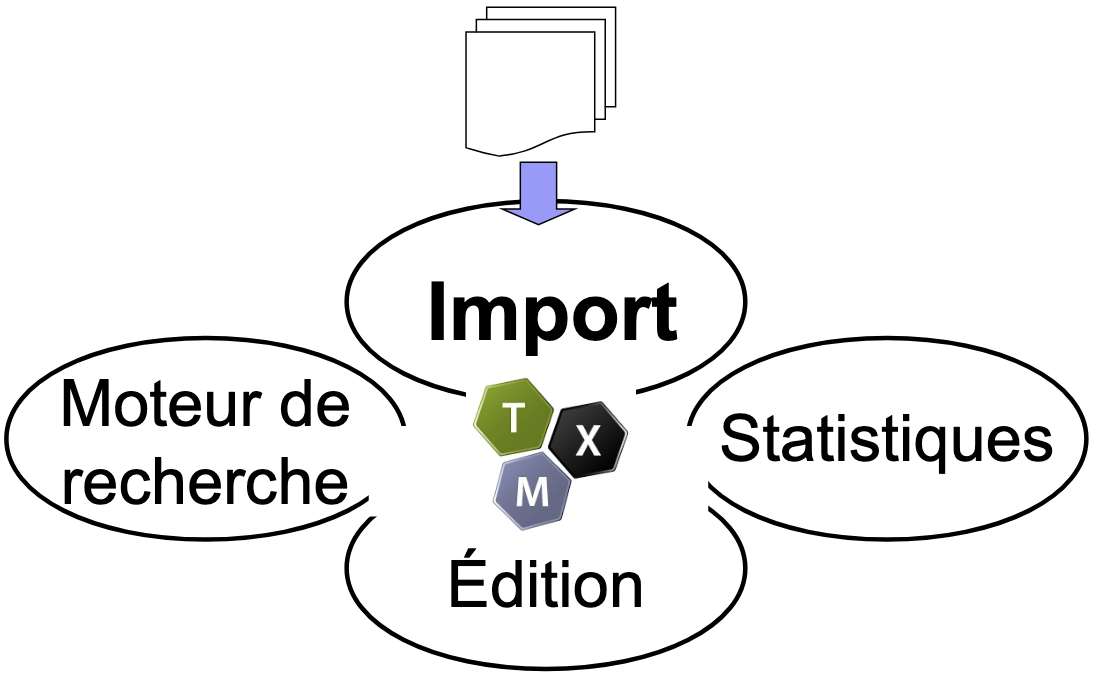
\includegraphics[width=1\linewidth]{img/import_txm.png}
		\caption{Schéma basique du \textit{workflow} dans \texttt{TXM} \citep{heiden}.}
		\label{fig:ling_out_TAL}
	\end{figure}
\end{frame}




\begin{frame}{Import du corpus}
	\begin{figure}[h] % Use [H] to force the figure to stay in place
		\centering
		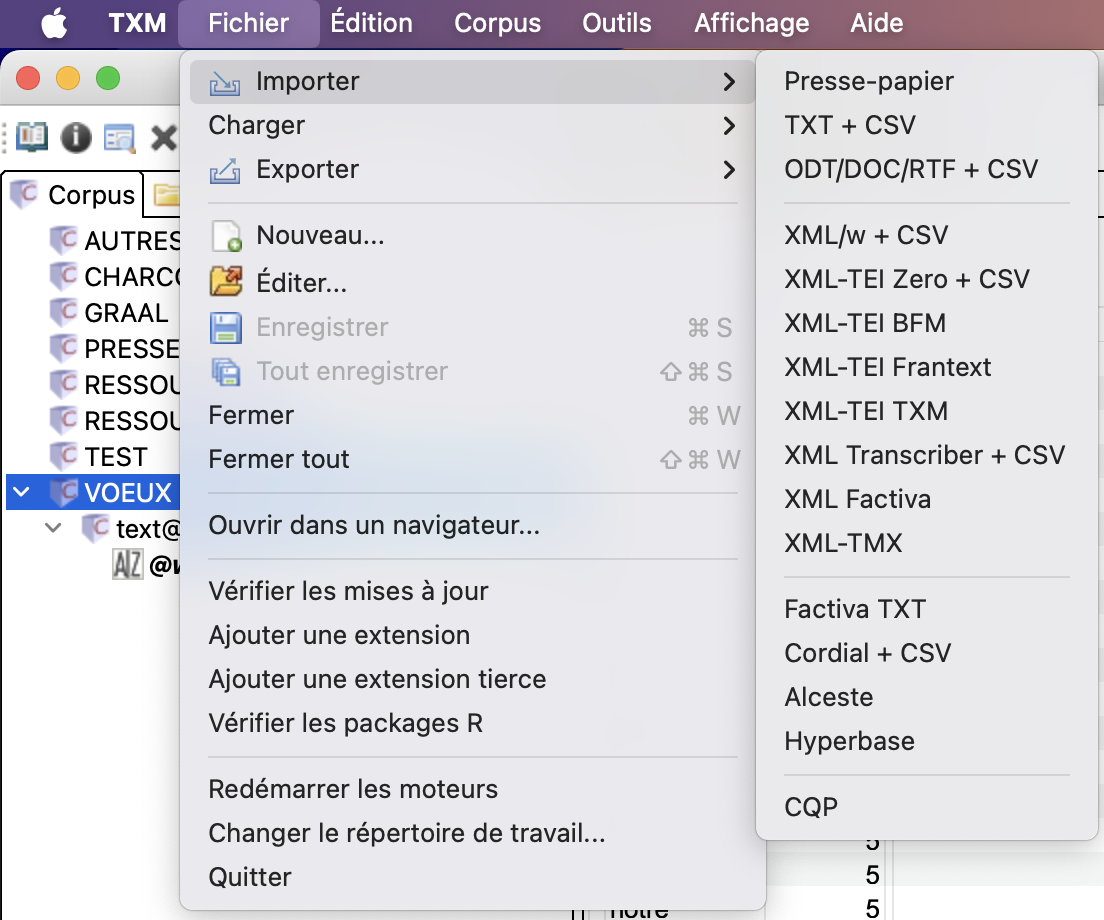
\includegraphics[width=0.7\linewidth]{img/import_corpus.png}
		\caption{Options d'import du corpus aux différents formats.}
		\label{fig:ling_out_TAL}
	\end{figure}
\end{frame}


\begin{frame}{Niveaux d'import}
	\begin{figure}[h] % Use [H] to force the figure to stay in place
		\centering
		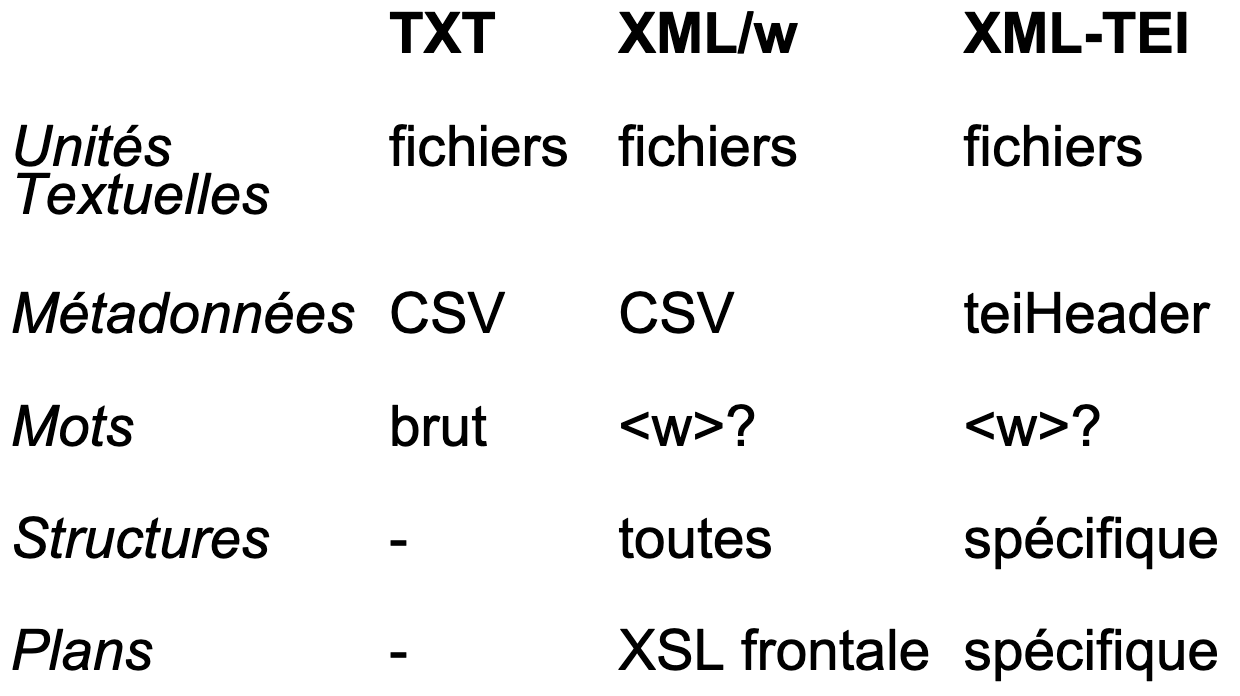
\includegraphics[width=.8\linewidth]{img/niveaux_import_txm.png}
		\caption{Carte des niveaux d'import \texttt{TXM} \citep{heiden}.}
		\label{fig:ling_out_TAL}
	\end{figure}
\end{frame}

\begin{frame}{Paramètres d'importation du corpus}
		\begin{figure}[h] % Use [H] to force the figure to stay in place
		\centering
		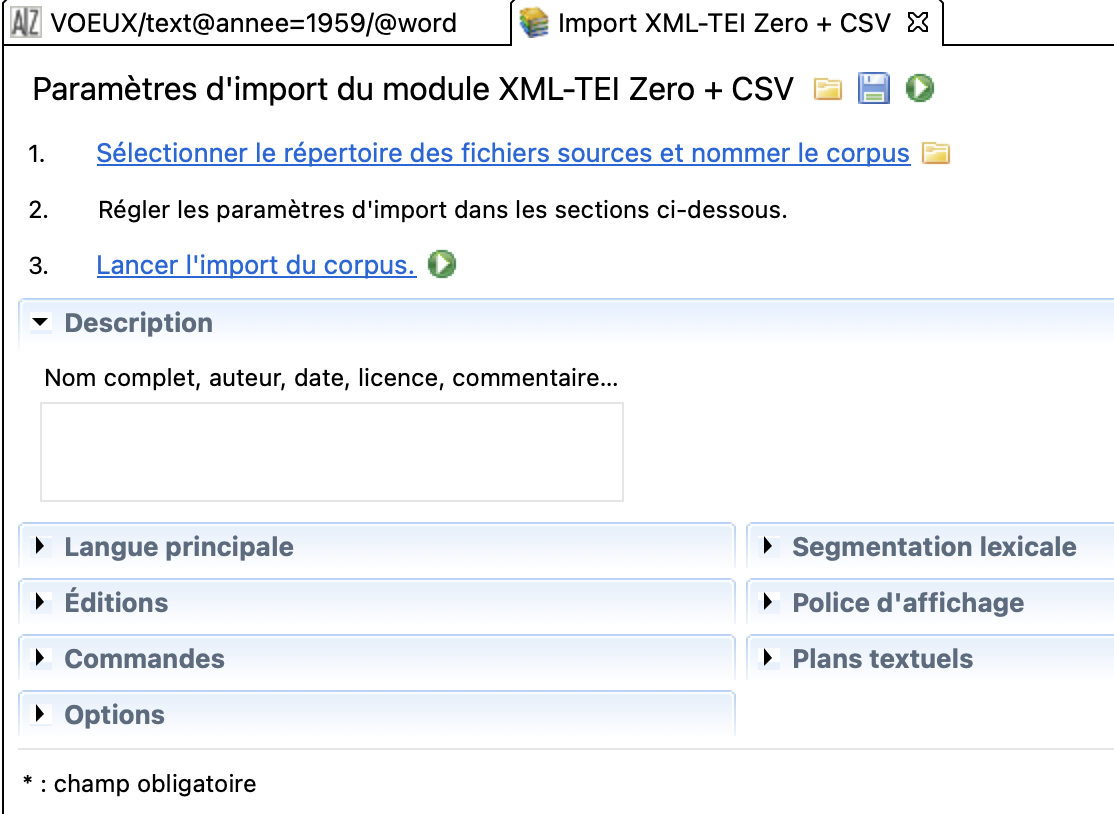
\includegraphics[width=0.8\linewidth]{img/preparation_import.png}
		\caption{Préparation de l'importation du corpus.}
		\label{fig:ling_out_TAL}
	\end{figure}
\end{frame}

\begin{frame}{Pourquoi structurer un document ?}
	La structuration permet de :
	\begin{itemize}
		\item expliciter pour la machine
		\item exploiter la dynamique interne du corpus
	\end{itemize} 
	
	Contraignant mais permet d'utiliser les fonctions avancées
	qui tirent partie des sous-corpus (donc des meta-données)
\end{frame}

\begin{frame}{Exemple de problème de structuration}
			\begin{figure}[h] % Use [H] to force the figure to stay in place
		\centering
		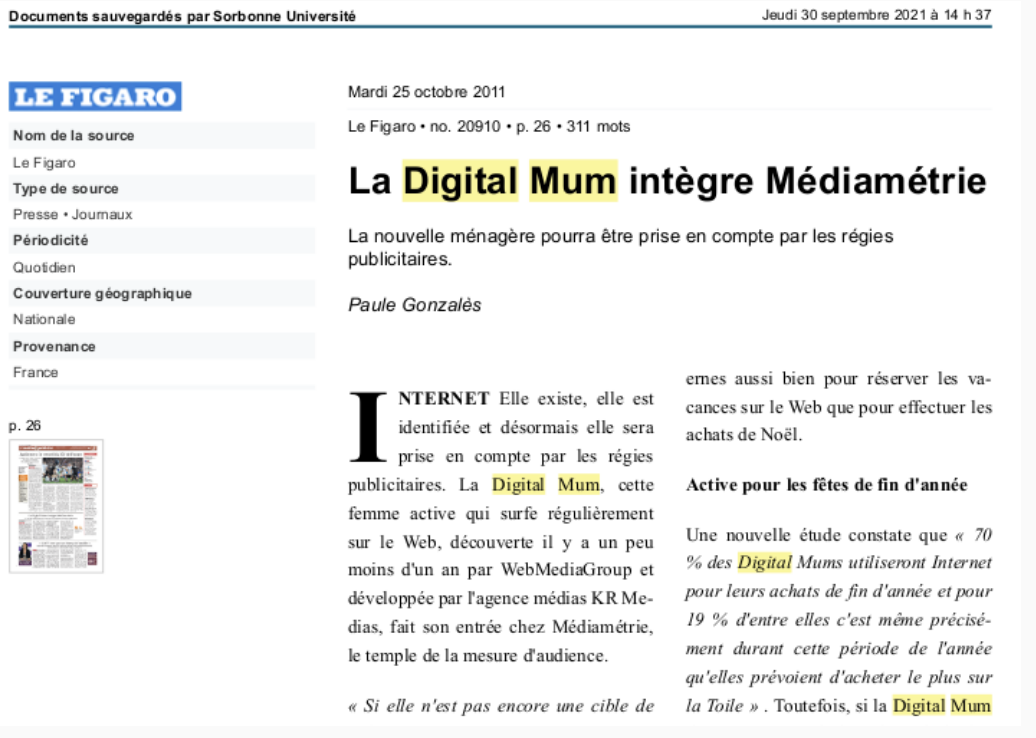
\includegraphics[width=.8\linewidth]{img/structuration.png}
		\caption{Problème de structuration \citep{lejeune2023}.}
		\label{fig:ling_out_TAL}
	\end{figure}
\end{frame}

\begin{frame}{Exemple de données structurées}
	\begin{figure}[h] % Use [H] to force the figure to stay in place
		\centering
		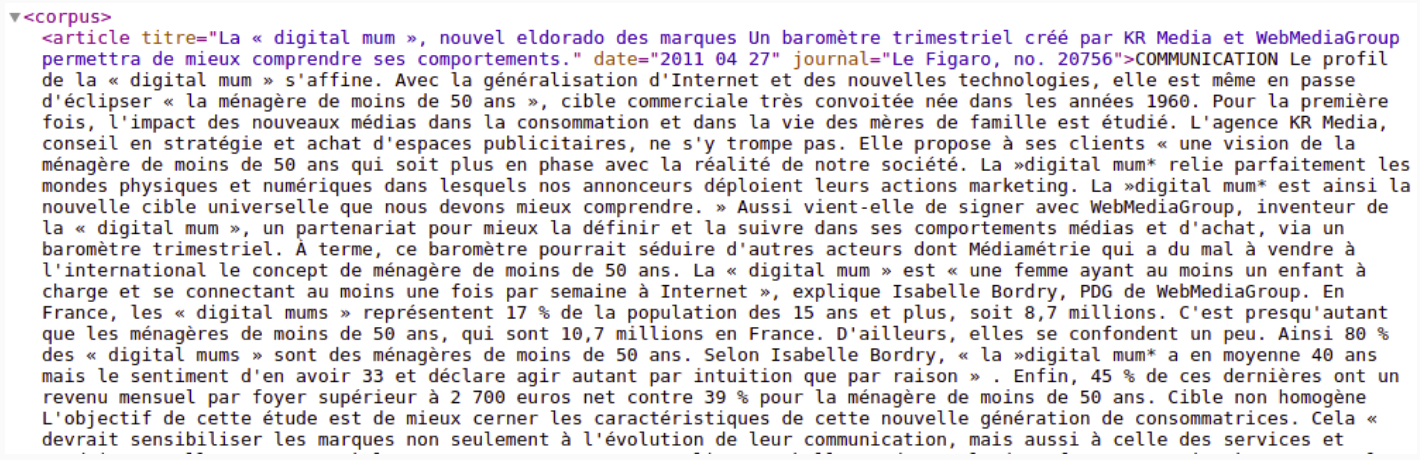
\includegraphics[width=1\linewidth]{img/structure.png}
		\caption{Problème de structuration \citep{lejeune2023}.}
		\label{fig:ling_out_TAL}
	\end{figure}
\end{frame}

\begin{frame}{\textsc{XML}}
	
	{\small angl. \textit{eXtensible Markup Language}}
	\begin{itemize}
		\item langage informatique de \textbf{balisage} (comme \textsc{HTML} ou \textsc{SGML})
		\item \textbf{textuel}, \textbf{structuré}, et \textbf{extensible}
		\begin{itemize}
					\item son \og{}langage\fg{} (vocabulaire et grammaire) peut être redéfini (p. ex., \texttt{mabalise} peut être un nom de balise)
			\item \textbf{syntaxe} stricte, peut être validée par des outils automatiques
		\end{itemize} 
	\end{itemize}
\end{frame}

\begin{frame}{Exemple du fichier \textsc{XML}}
	\textit{Cf.} le tutoriel \textsc{W3C}\footnote{\url{https://www.w3schools.blog/xml-tutorial}.}
	   \begin{figure}[ht]
		\begin{minipage}[b]{0.45\linewidth}
			\centering
			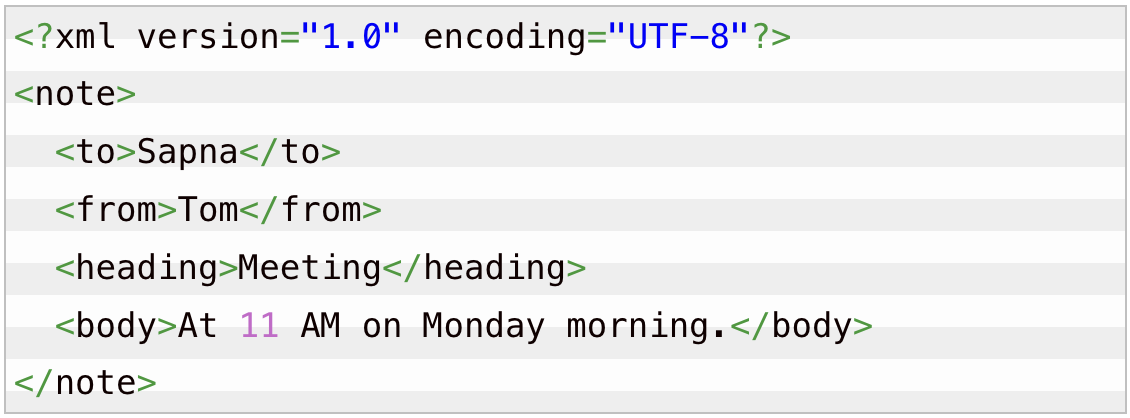
\includegraphics[width=\textwidth]{img/xml_note_xml.png}
			\caption{Exemple d'un fichier \textsc{XML}.}
			\label{fig:a}
		\end{minipage}
		\hspace{0.5cm}
		\begin{minipage}[b]{0.45\linewidth}
			\centering
			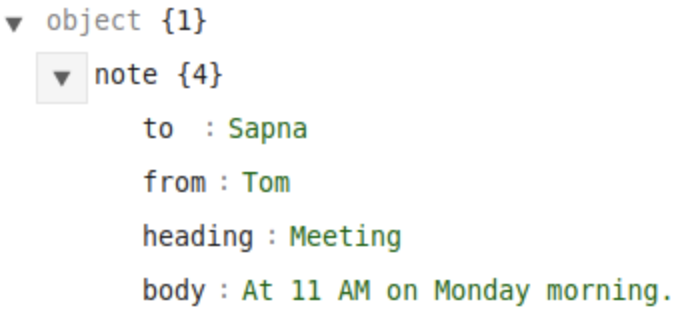
\includegraphics[width=\textwidth]{img/xml_note.png}
			\caption{Exemple de la structure arborescente du fichier \textsc{XML}.}
			\label{fig:b}
		\end{minipage}
	\end{figure}
\end{frame}

\begin{frame}{\textsc{TEI}}

{\small angl. \textit{Text Encoding Initiative}\footnote{\url{http://www.tei-c.org}}} (depuis 1987)

Consortium à but non lucratif :
\begin{itemize}
	\item auto-financé
	\item institutions, projets de recherche et chercheurs
	\item \bolder{standard pour la représentation des textes
	numériques}
	\begin{itemize}
		\item un format \textsc{SGML} au début, \textsc{XML} maintenant
		\end{itemize}
	\item documentation, outils et formations
\end{itemize}
\end{frame}

\begin{frame}{Exemple du document \textsc{XML-TEI}}
		\begin{figure}[h] % Use [H] to force the figure to stay in place
		\centering
		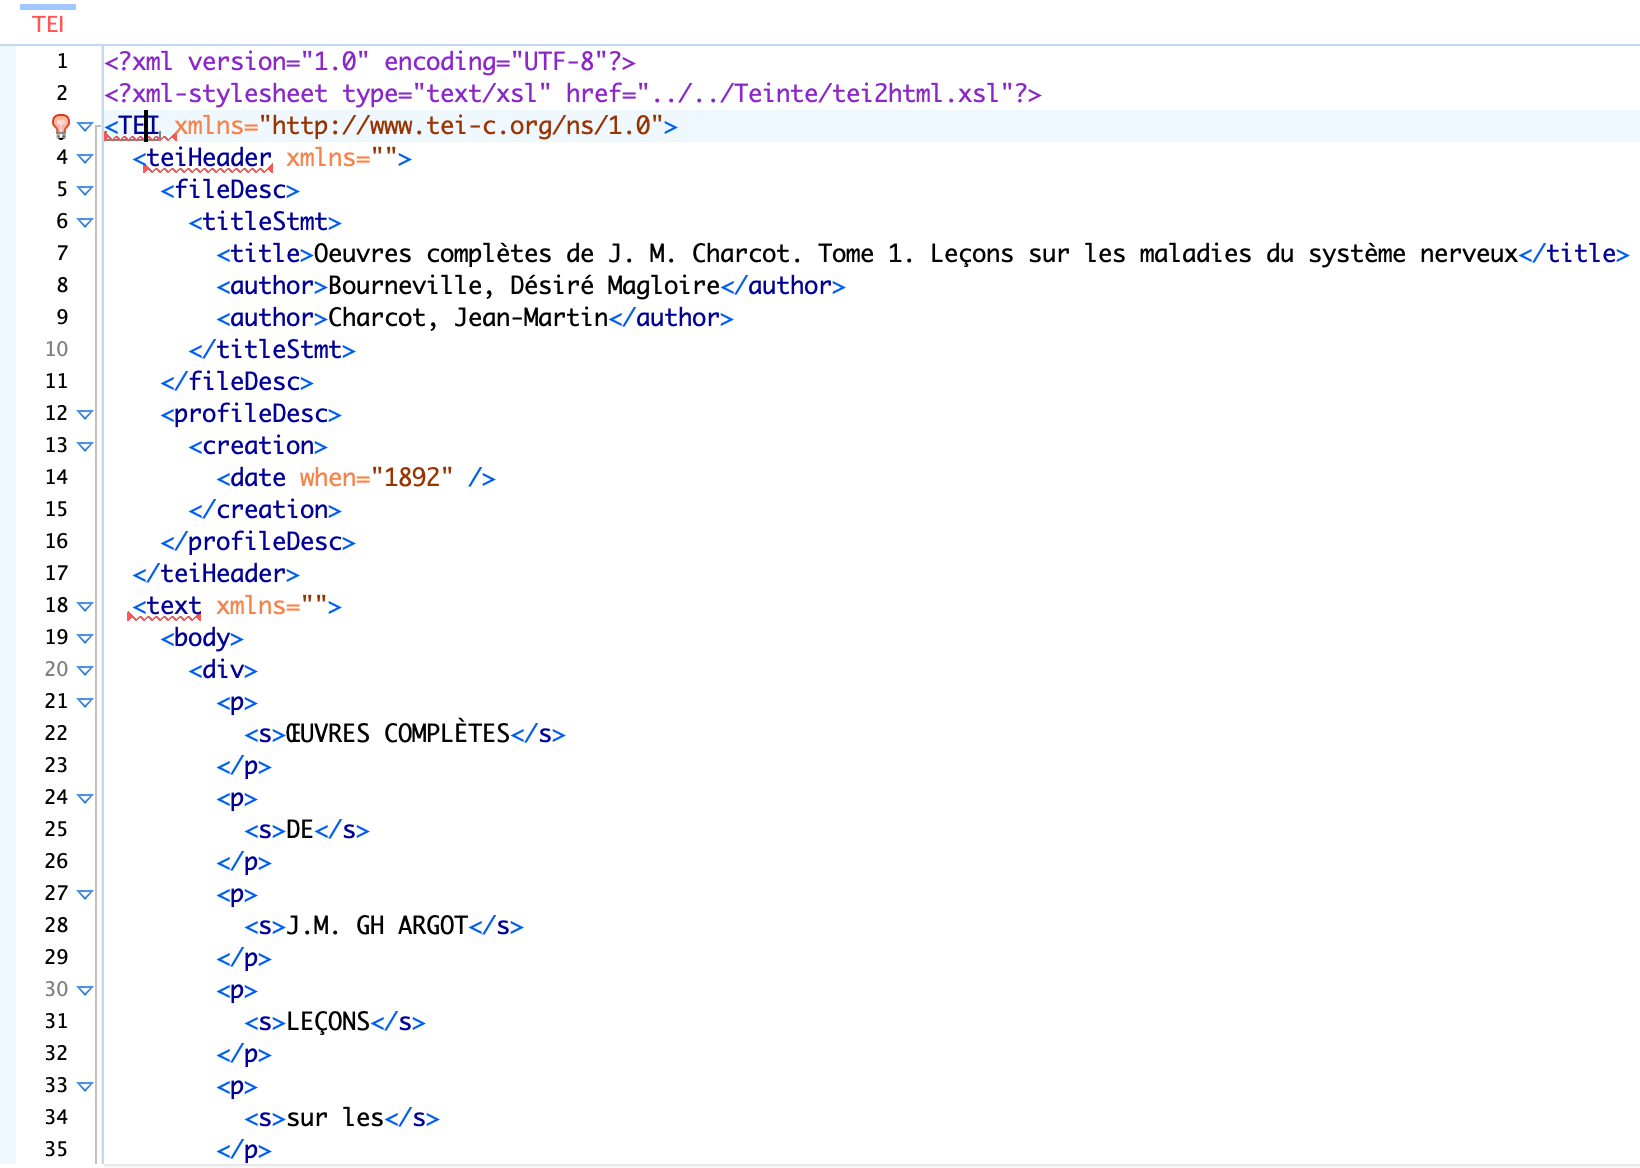
\includegraphics[width=.9\linewidth]{img/charcot_tei.png}
		\caption{Corpus \texttt{CHARCOT} au format \textsc{XML-TEI}.}
		\label{fig:ling_out_TAL}
	\end{figure}
\end{frame}

\begin{frame}{Exemple du document \textsc{XML-TEI} : mode édition}
	\begin{figure}[h] % Use [H] to force the figure to stay in place
		\centering
		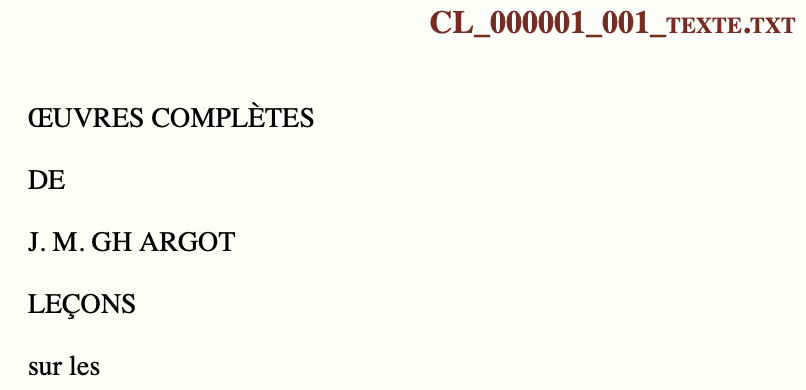
\includegraphics[width=1\linewidth]{img/charcot_tei_edition.png}
		\caption{Corpus \texttt{CHARCOT} au format \textsc{XML-TEI} : mode édition.}
		\label{fig:ling_out_TAL}
	\end{figure}
\end{frame}

\begin{frame}{Métadonnées}
	\og{}des données sur les données\fg{}
	
	Les métadonnées doivent être décrites quelque part.
	\begin{itemize}
		\item fichier \texttt{metadata.csv} (dans le répertoire du corpus)
		\item à l'import, \textsc{TXM} associe chaque texte du corpus à ses métadonnées
	\end{itemize}
\end{frame}

\begin{frame}{Exemple de fichier \texttt{metadata.csv}, corpus \texttt{VOEUX}}
		\begin{figure}[h] % Use [H] to force the figure to stay in place
		\centering
		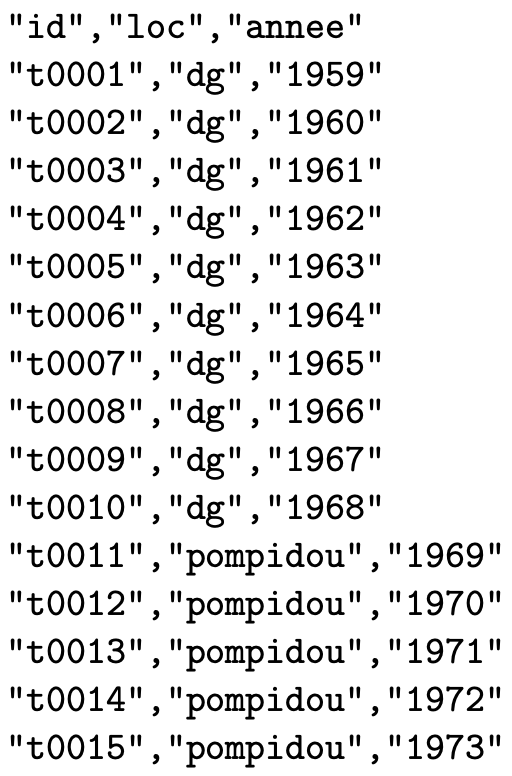
\includegraphics[width=.4\linewidth]{img/metadata_csv.png}
		\caption{Identifiants, locuteurs (ex. \texttt{dg} : De Gaulle), année.}
		\label{fig:ling_out_TAL}
	\end{figure}
\end{frame}
\section{Autres fonctionnalités \texttt{TXM}}

\begin{frame}{Progression}
		\begin{block}{\vspace{-6mm}}
		\justifying
 Graphique cumulative de l'évolution d'un ou de plusieurs motifs au fil d'un corpus, exprimés par des requêtes \textsc{CQL}.
 \end{block}
 
{\small \texttt{T} : total général (nombre de mots dans le corpus)\\ \texttt{Occurrences} : fréquences générales dans le corpus}

	\begin{figure}[h] % Use [H] to force the figure to stay in place
		\centering
		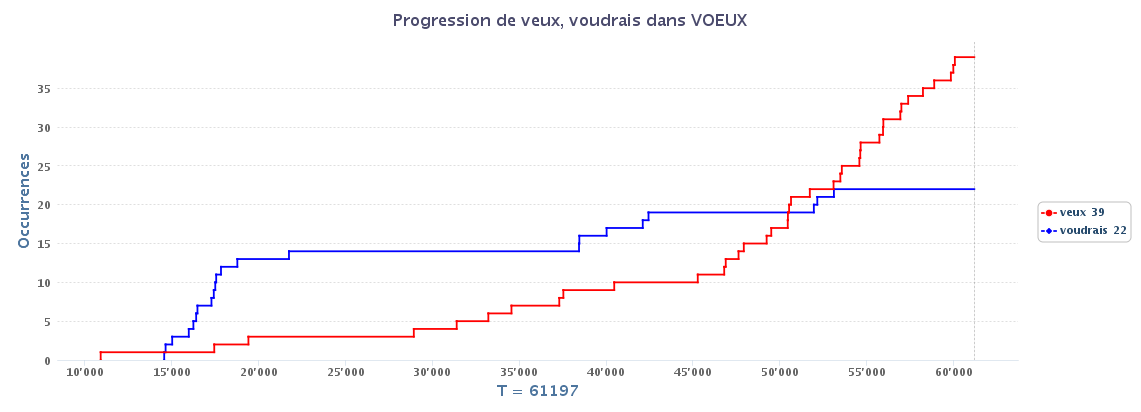
\includegraphics[width=.9\linewidth]{img/progression.png}
		\caption{Évolution des formes verbales, exemple de \textcite{lejeune2023}.}
		\label{fig:ling_out_TAL}
	\end{figure}
\end{frame}

\begin{frame}{Progression}
	\begin{itemize}
		\item Utilisation des étiquettes \textsc{POS}
	\end{itemize}
	\begin{figure}[h] % Use [H] to force the figure to stay in place
		\centering
		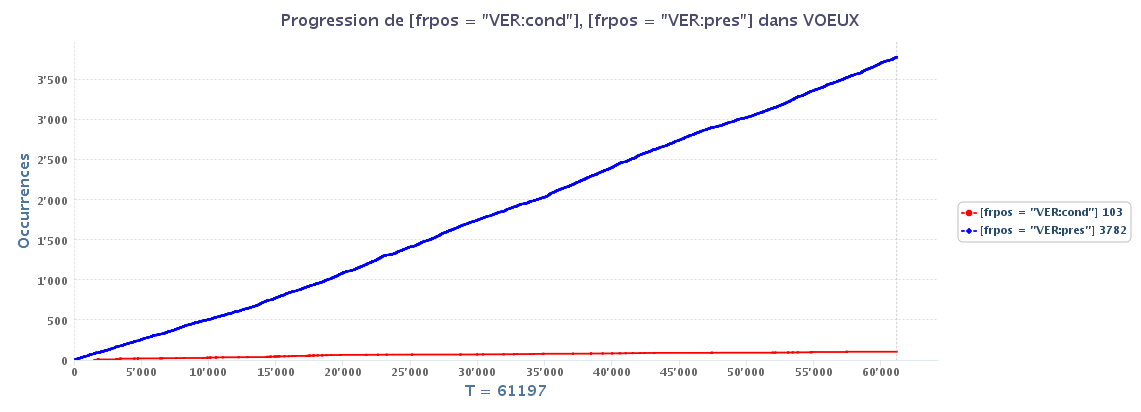
\includegraphics[width=1\linewidth]{img/ver_cond_pres.png}
		\caption{Évolution des formes verbales \textit{veux} (prés.) et \textit{voudrais} (cond.) à l'aide des étiquettes \textsc{POS}, exemple de \textcite{lejeune2023}.}
		\label{fig:ling_out_TAL}
	\end{figure}
\end{frame}

\section{Comparer au sein d'un corpus}

\begin{frame}{Création de sous-corpus et de partitions}
		\begin{figure}[h] % Use [H] to force the figure to stay in place
		\centering
		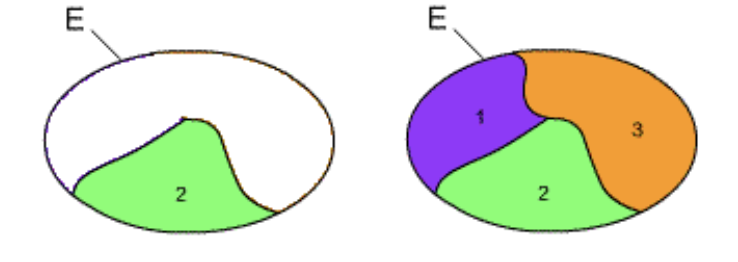
\includegraphics[width=.5\linewidth]{img/partition_sous-corpus.png}
		\caption{Sous-corpus \textit{vs.} partitions dans un ensemble \texttt{E}, adapté de \textcite{fort}.}
		\label{fig:ling_out_TAL}
	\end{figure}
	\begin{itemize}
		\item \bolder{sous-corpus} : regroupement \og{}minimal\fg{} déterminé selon les métadonnées, sélection d'une partie de l'ensemble sans contrainte
		\item \bolder{partition} : un ensemble de sous-corpus, divise tout l'ensemble en parties disjointes et exhaustives
	\end{itemize}
	On peut ensuite \og{}opposer\fg{} des partitions pour faire émerger des	phénomènes par contraste.
 
\end{frame}

\begin{frame}{Exemple de création de partition}
Créer une partition du corpus \texttt{VOEUX} selon le locuteur \texttt{MITTERRAND}.

   \begin{figure}[ht]
	\begin{minipage}[b]{0.45\linewidth}
		\centering
		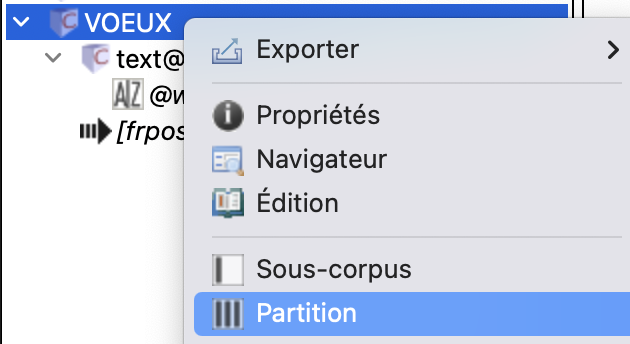
\includegraphics[width=\textwidth]{img/partition.png}
		\caption{Création de la partition.}
		\label{fig:a}
	\end{minipage}
	\hspace{0.5cm}
	\begin{minipage}[b]{0.45\linewidth}
		\centering
		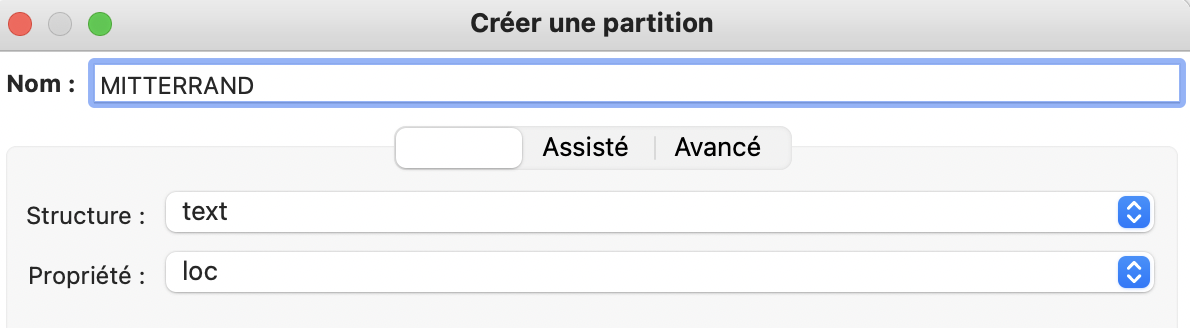
\includegraphics[width=\textwidth]{img/partition_mitterrand.png}
		\caption{Choix du locuteur François Mitterrand}
		\label{fig:b}
	\end{minipage}
\end{figure}

%		\begin{figure}[h] % Use [H] to force the figure to stay in place
%	\centering
%	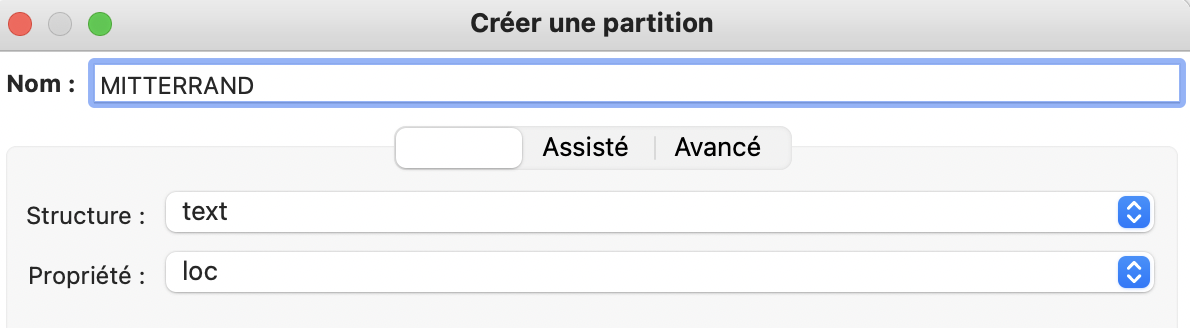
\includegraphics[width=.5\linewidth]{img/partition_mitterrand.png}
%	\caption{Partition dédié au locuteur François Mitterrand.}
%	\label{fig:ling_out_TAL}
%\end{figure}
\end{frame}

\begin{frame}{Dimensions de la partition}
	\begin{figure}[h] % Use [H] to force the figure to stay in place
		\centering
		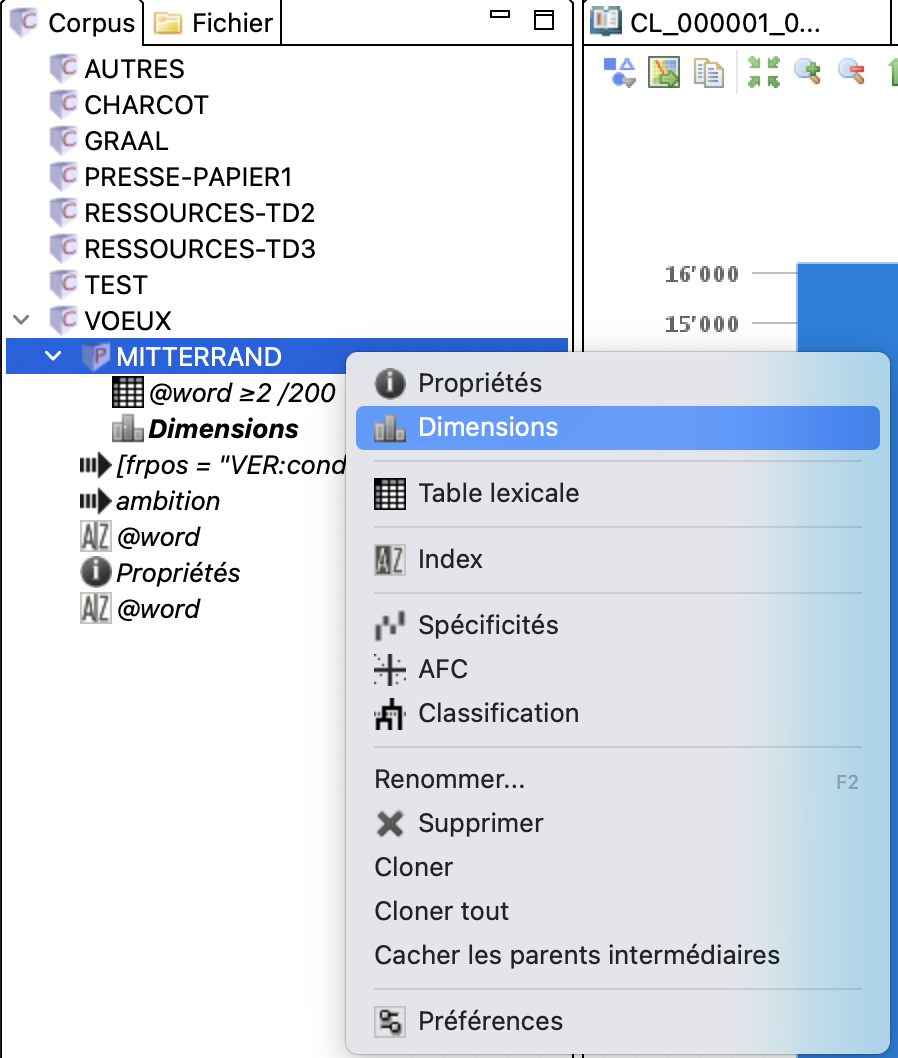
\includegraphics[width=.5\linewidth]{img/dimensions.png}
		\caption{Dimension d'une partition.}
		\label{fig:ling_out_TAL}
	\end{figure}
\end{frame}

\begin{frame}{Dimensions de la partition}
			\begin{figure}[h] % Use [H] to force the figure to stay in place
		\centering
		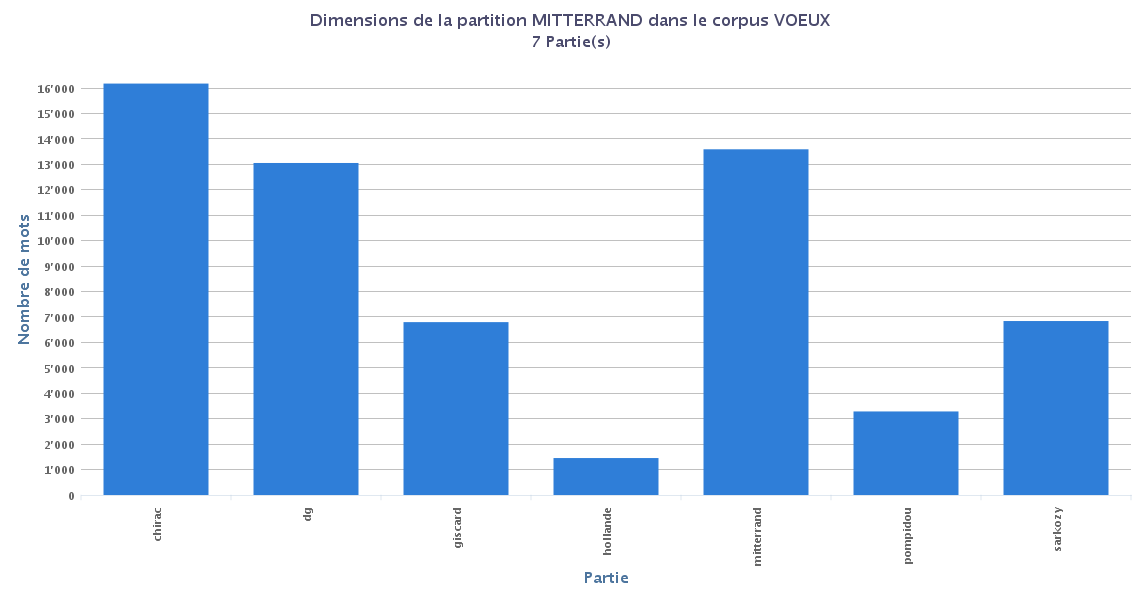
\includegraphics[width=1\linewidth]{img/dimensions_mitterrand.png}
		\caption{Dimension de la partition \texttt{MITTERRAND} dans le corpus \texttt{VOEUX}.}
		\label{fig:ling_out_TAL}
	\end{figure}
\end{frame}

\begin{frame}{Progression}
	\begin{figure}[h] % Use [H] to force the figure to stay in place
		\centering
		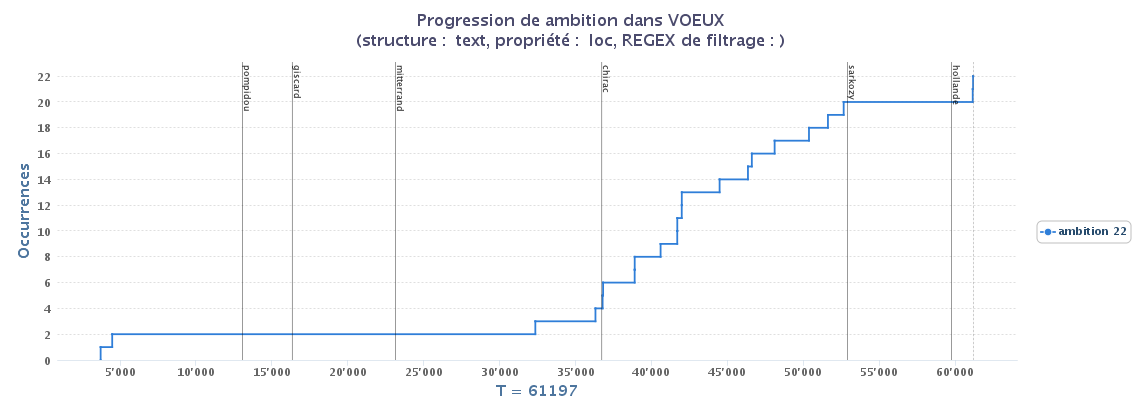
\includegraphics[width=1\linewidth]{img/ambition.png}
		\caption{Évolution du terme \textit{ambition} dans les partitions du corpus \texttt{VOEUX}.}
		\label{fig:ling_out_TAL}
	\end{figure}
\end{frame}

\begin{frame}{Table lexicale}
		\begin{figure}[h] % Use [H] to force the figure to stay in place
		\centering
		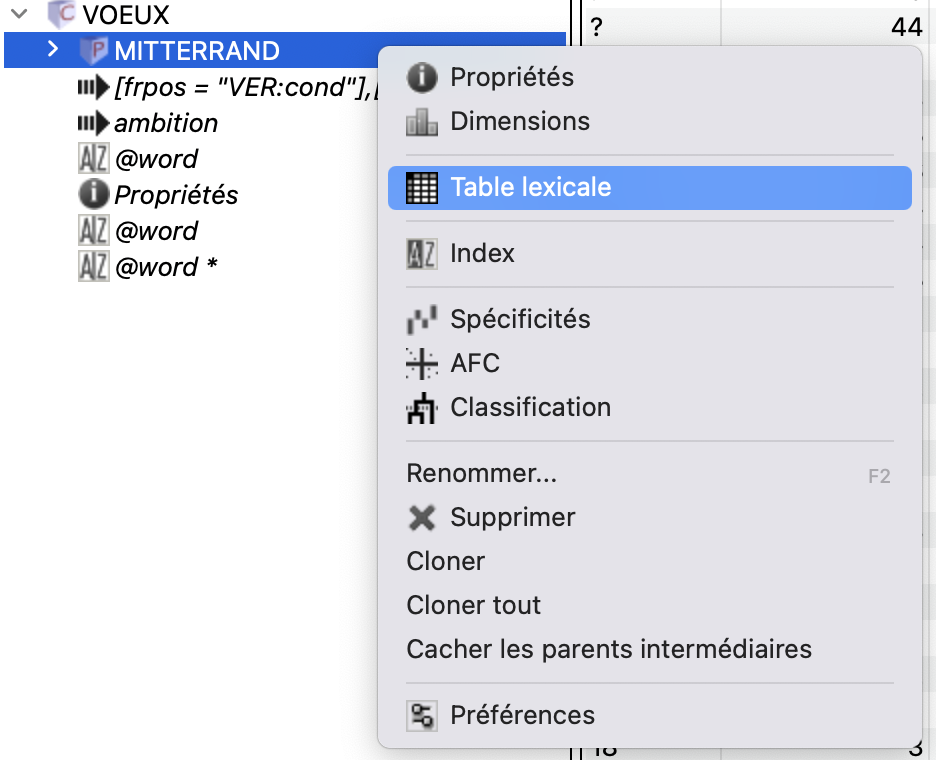
\includegraphics[width=.7\linewidth]{img/table_lexicale.png}
		\caption{Générer une table lexicale pour toutes les partitions.}
		\label{fig:ling_out_TAL}
	\end{figure}
\end{frame}

\begin{frame}{Table lexicale}
	\begin{block}{\vspace{-6mm}}
		\begin{itemize}
				\item les fréquences brutes sont biaisées par la taille des parties
				\item les spécificités de Lafon permettent de rendre les comparaisons plus fiables en ajustant les fréquences en fonction des tailles relatives des sous-corpus
		\end{itemize}
	\end{block}
	\begin{itemize}
		\item \texttt{T} : total général (nombre de mots)
		\item \texttt{t} : total dans la partie (nombre de mots)
	\end{itemize}
	 
	\begin{figure}[h] % Use [H] to force the figure to stay in place
		\centering
		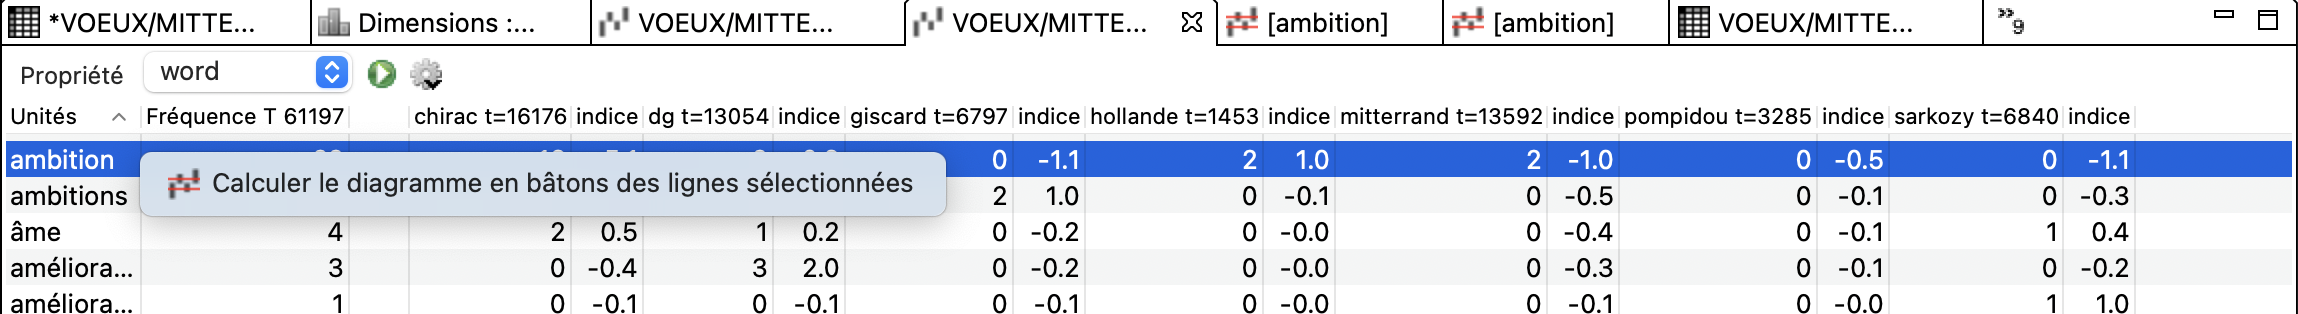
\includegraphics[width=1\linewidth]{img/diagramme_batons.png}
		\caption{Générer le diagramme en bâtons pour le terme \textit{ambition} dans toutes les partitions.}
		\label{fig:ling_out_TAL}
	\end{figure}
\end{frame}

\begin{frame}{Calcul de spécificités \citep{lafon1980variabilite}}
	\begin{block}{\vspace{-6mm}}
		\justifying
		\begin{itemize}
			\item mesure le caractère attendu ou exceptionnel de la fréquence
			d’un mot (ou motif complexe, trait linguistique, etc.) dans une partie du corpus, au regard de sa
			fréquence dans l’ensemble du corpus et de la taille de la partie
		\end{itemize}
	\end{block}
	
	Calcul qui ne nécessite que 4 variables :
	\begin{itemize}
		\item \texttt{T} (total général)
		\item \texttt{t} (total dans la partie)
		\item \texttt{F} (fréquence générale)
		\item \texttt{f} (fréquence dans la partie)
	\end{itemize}
\end{frame}

\begin{frame}{Spécificités}
	Est-ce que la fréquence du mot est étonnante
	par rapport à la probabilité attendue ?
	\begin{figure}[h] % Use [H] to force the figure to stay in place
	\centering
	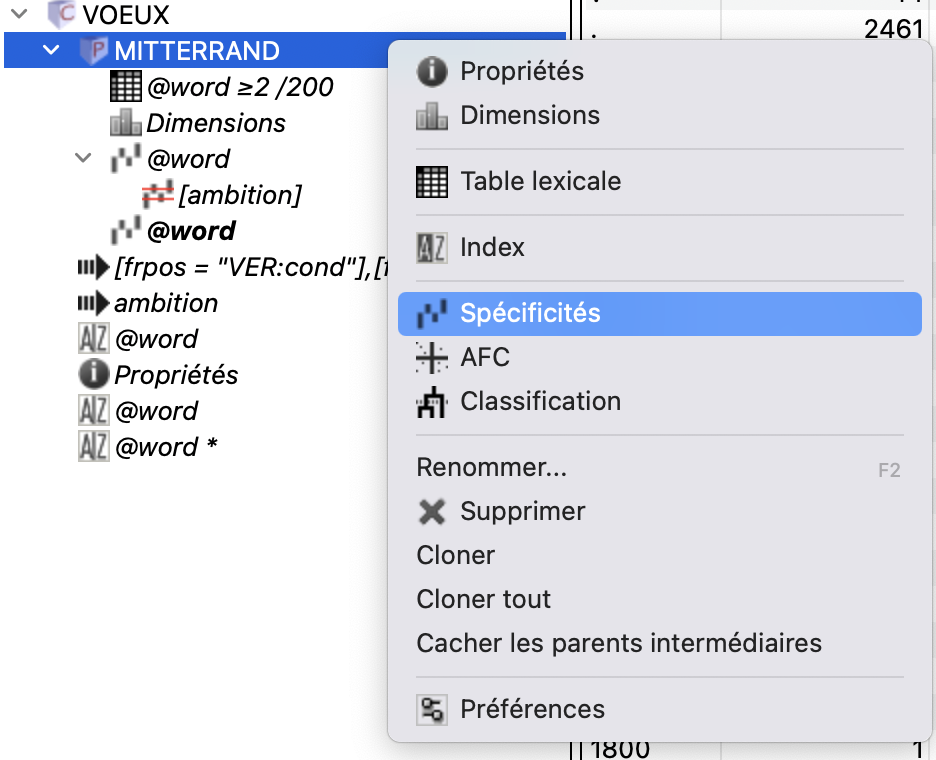
\includegraphics[width=.6\linewidth]{img/specificites.png}
	\caption{Calcul des spécificités.}
	\label{fig:ling_out_TAL}
\end{figure}
\end{frame}

\begin{frame}{Spécificités}
	\begin{figure}[h] % Use [H] to force the figure to stay in place
		\centering
		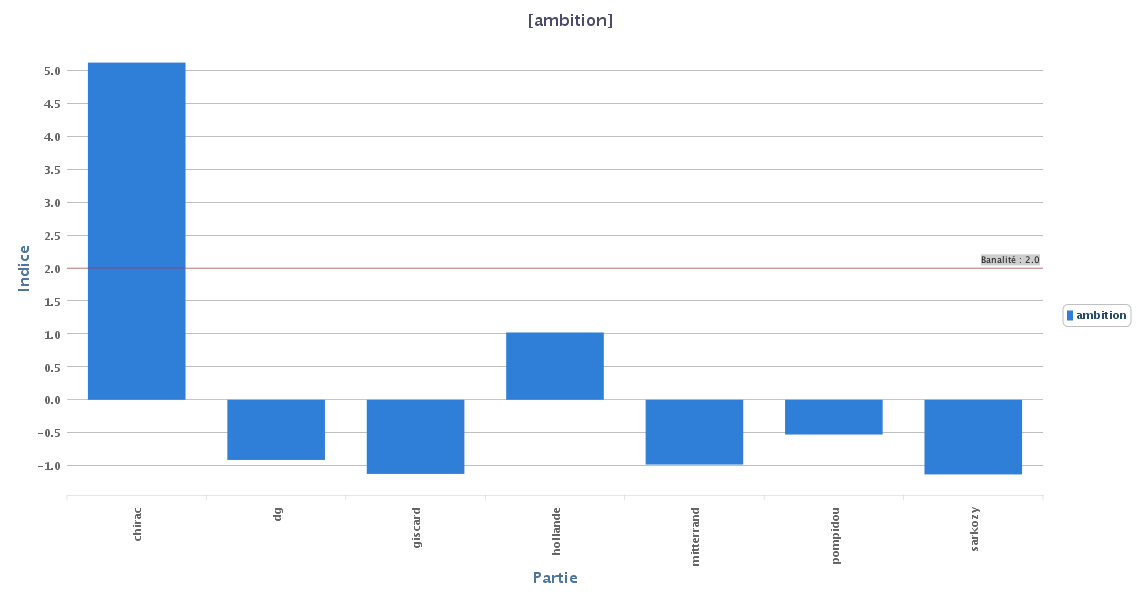
\includegraphics[width=1\linewidth]{img/ambition_specificites.png}
		\caption{Indice de spécificité pour le mot \textit{ambition} dans les différentes partitions du corpus \texttt{VOEUX}.}
		\label{fig:ling_out_TAL}
	\end{figure}
\end{frame}

\begin{frame}{Spécificités}
	\begin{figure}[h] % Use [H] to force the figure to stay in place
		\centering
		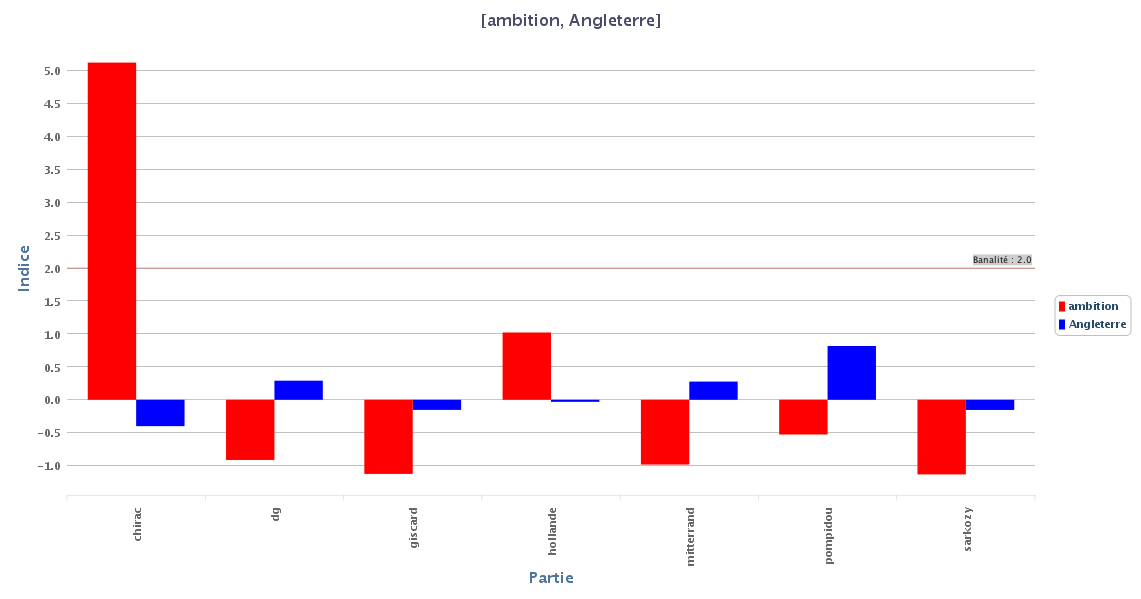
\includegraphics[width=1\linewidth]{img/ambition_angleterre.png}
		\caption{Indices de spécificité pour les mots \textit{ambition} et \textit{Angleterre} dans les différentes partitions du corpus \texttt{VOEUX}.}
		\label{fig:ling_out_TAL}
	\end{figure}
\end{frame}

\begin{frame}{Interprétation}
	\begin{itemize}
		\item chaque partie est représentée par un ensemble de barres contiguës, classées dans le
		même ordre que dans le tableau
		\item chaque propriété de mot (forme graphique) sera représentée
		par une barre de la même couleur dans chaque partie
		\item les couleurs sont légendées dans le coin inférieur droit du graphique
		\item la ligne rouge délimite la \bolder{zone de banalité} autour de l'axe d'indice 2 
		\begin{itemize}
			\item les barres qui n'en sortent pas sont à considérer comme banales
		\end{itemize}
		\end{itemize}
\end{frame}
\begin{frame}{Interprétation}
\begin{itemize}
\item zone de banalité représentée sur le graphique pour éviter de surinterpréter
\begin{itemize}
\item banalité (forte probabilité) de l'apparition dans la partie 
\item mots prévisibles d'après le modèle des spécificités
\end{itemize}
\item une significativité négative peut avoir du sens : \bolder{nullax}
\begin{itemize}
	\item mots ayant un indice négatif mais aussi une fréquence nulle
	\item mots dont l’absence dans la partie est statistiquement
	étonnante, compte tenu de sa fréquence en corpus et de la taille de la partie 
\end{itemize}
\end{itemize}
\begin{flushright}
	{\small \citep{pincemin2022semantique}}
\end{flushright}
\end{frame}



\begin{frame}{Calcul des spécificités}
		Analogie de la boîte à \oe{}ufs :
	\begin{itemize}
		\item on renverse aléatoirement les \oe{}ufs (occurrences d'un mot) dans les boîtes à \oe{}ufs (partitions du corpus)
		\item rare que beaucoup d'œufs tombent dans une même boîte
		\item si les œufs sont répartis au hasard, ils devraient plutôt se distribuer plus uniformément entre les boîtes
	\end{itemize}
\end{frame}

\begin{frame}{Analyse factorielle des correspondances \citep{benzecri1973analyse}}
	\begin{itemize}
		\item synthèse globale des relations entre
		mots (traits linguistiques, motifs) et textes (parties du
		corpus) 
		\item les mots sont comparés les uns aux autres sur la base des textes qui les emploient
		\item et réciproquement les ressemblances et écarts entre textes sont évalués par le vocabulaire qu’ils
		mobilisent
	\end{itemize}
			\begin{figure}[h] % Use [H] to force the figure to stay in place
		\centering
		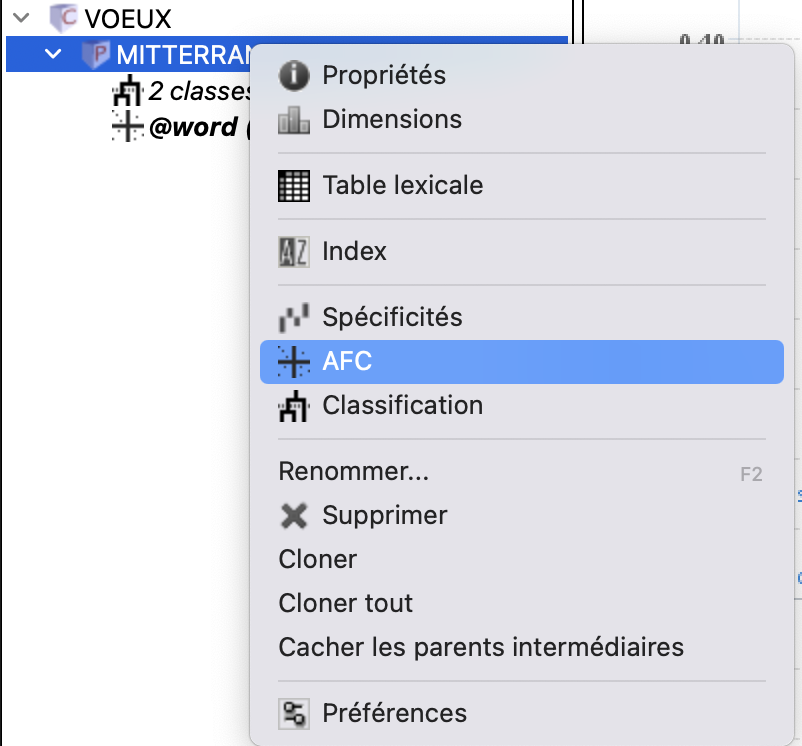
\includegraphics[width=.3\linewidth]{img/generer_afc.png}
		\caption{Générer l'analyse factorielle des correspondances.}
		\label{fig:ling_out_TAL}
	\end{figure}
\end{frame}
\begin{frame}{Analyse factorielle des correspondances -- corpus \texttt{VOEUX}}
		\begin{figure}[h] % Use [H] to force the figure to stay in place
		\centering
		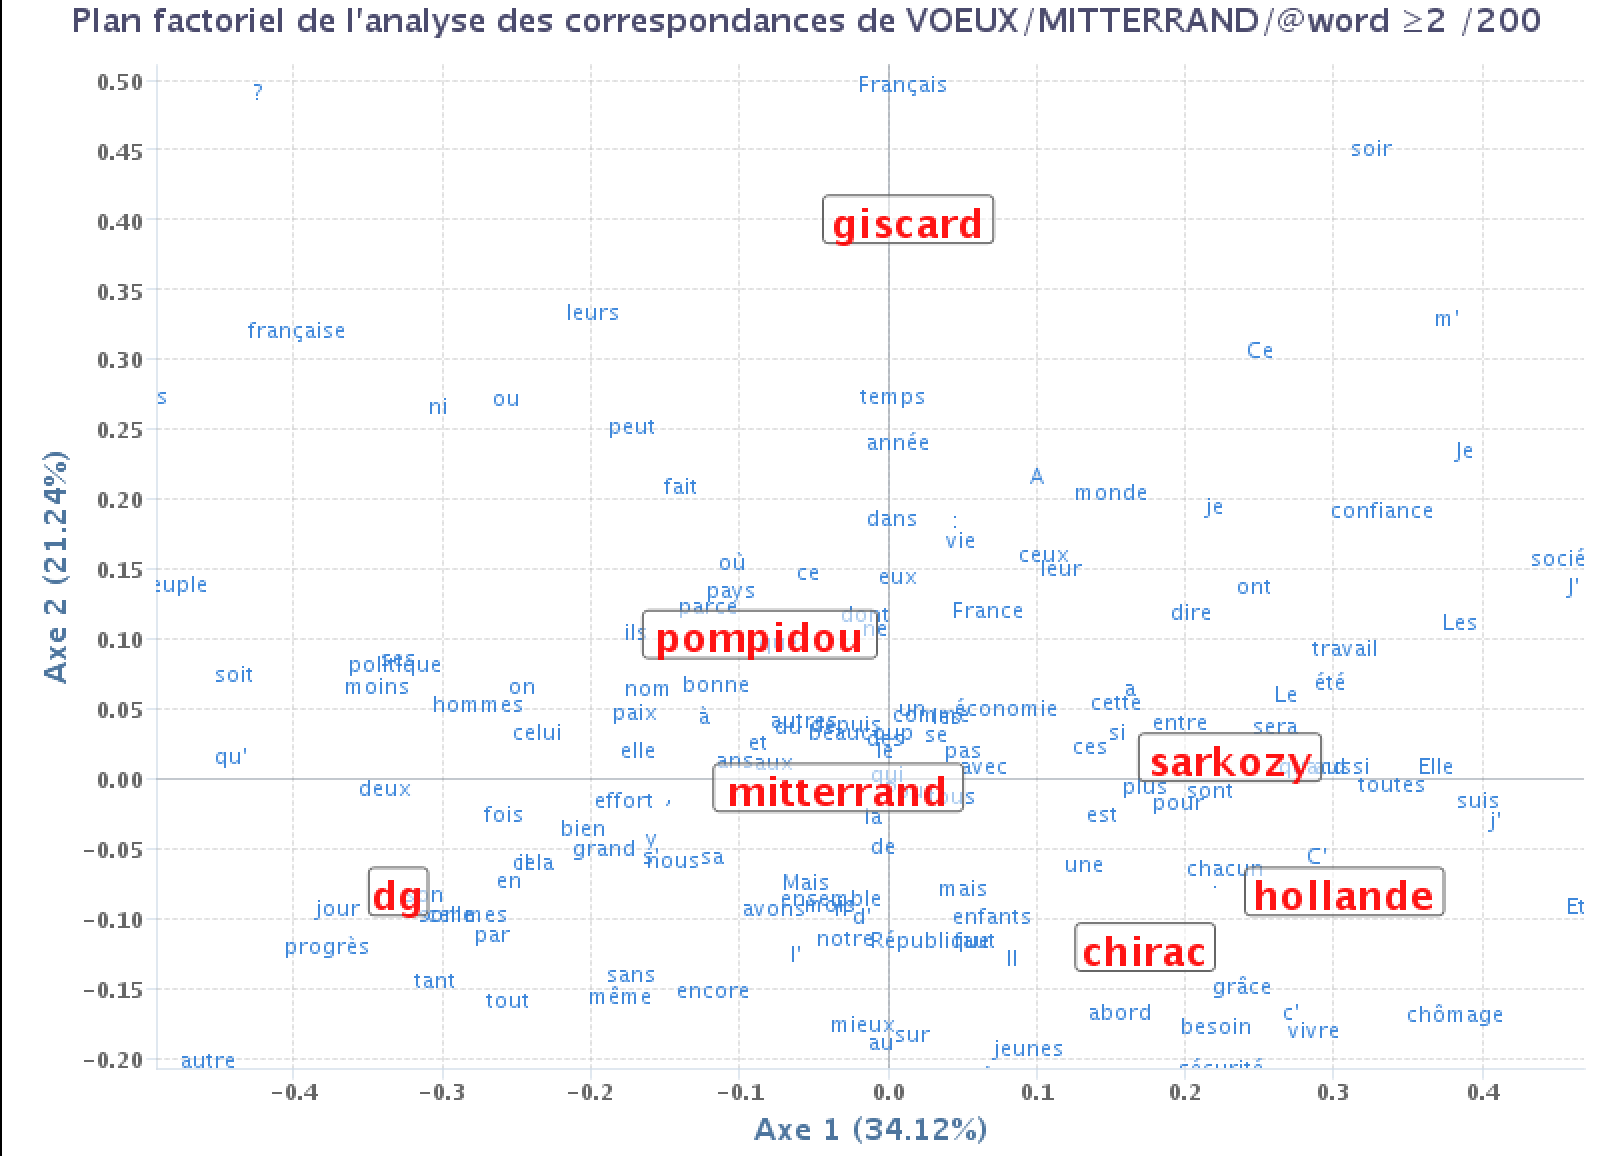
\includegraphics[width=.8\linewidth]{img/afc.png}
		\caption{Analyse factorielle des correspondances : représentation géométrique des présidents en lien avec une sélection de noms communs.}
		\label{fig:ling_out_TAL}
	\end{figure}
\end{frame}

\begin{frame}{Classification ascendante hiérarchique \citep{benzecri1979}}
		\begin{block}{\vspace{-6mm}}
		\justifying 
Méthode de rassemblement des éléments selon un critère de ressemblance défini au préalable qui s’exprimera sous la forme d’une matrice de distances.
		\end{block}
		\begin{itemize}
	\item le calcul s'effectue à partir des colonnes ou des lignes d'une table lexicale ou d’une partition	
\end{itemize}
			\begin{figure}[h] % Use [H] to force the figure to stay in place
		\centering
		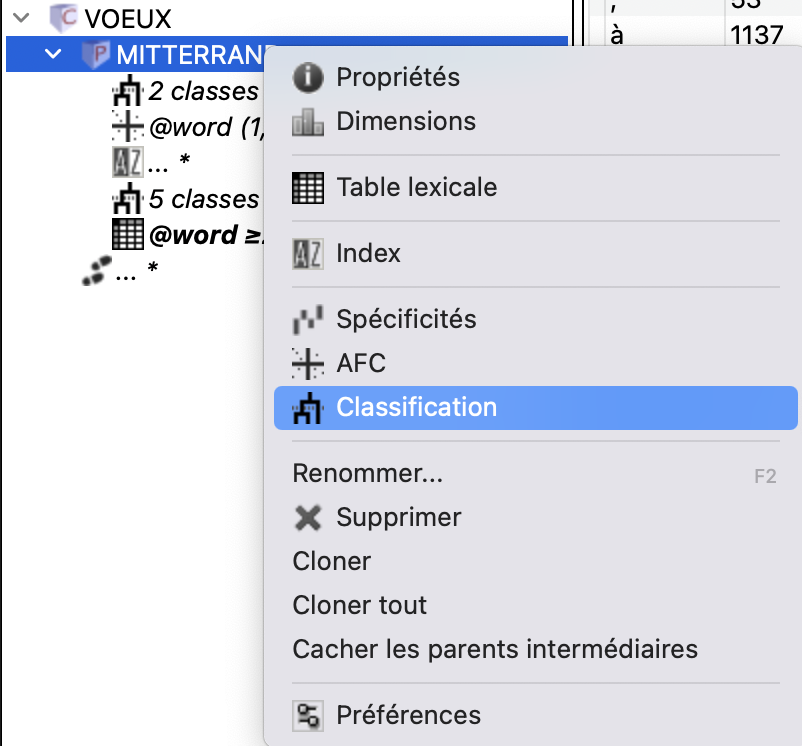
\includegraphics[width=.3\linewidth]{img/classif.png}
		\caption{Générer une classification ascendante hiérarchique.}
		\label{fig:ling_out_TAL}
	\end{figure}
\end{frame}

\begin{frame}{Visualisation de la classification ascendante hiérarchique}
Le dendrogramme avec des regroupements par classes d’éléments, composé de :
	\begin{itemize}
		\item de cadres de couleur correspondants aux regroupements par classes ;
		\item de l’échelle des indices de niveaux de regroupement située à gauche ;
	\end{itemize}
En haut à droite : le diagramme des indices de niveaux (du nœud le plus haut au nœud le plus bas du dendrogramme).


\end{frame}

\begin{frame}{Exemple de la \textsc{CAH} -- corpus \texttt{VOEUX}}
			\begin{figure}[h] % Use [H] to force the figure to stay in place
		\centering
		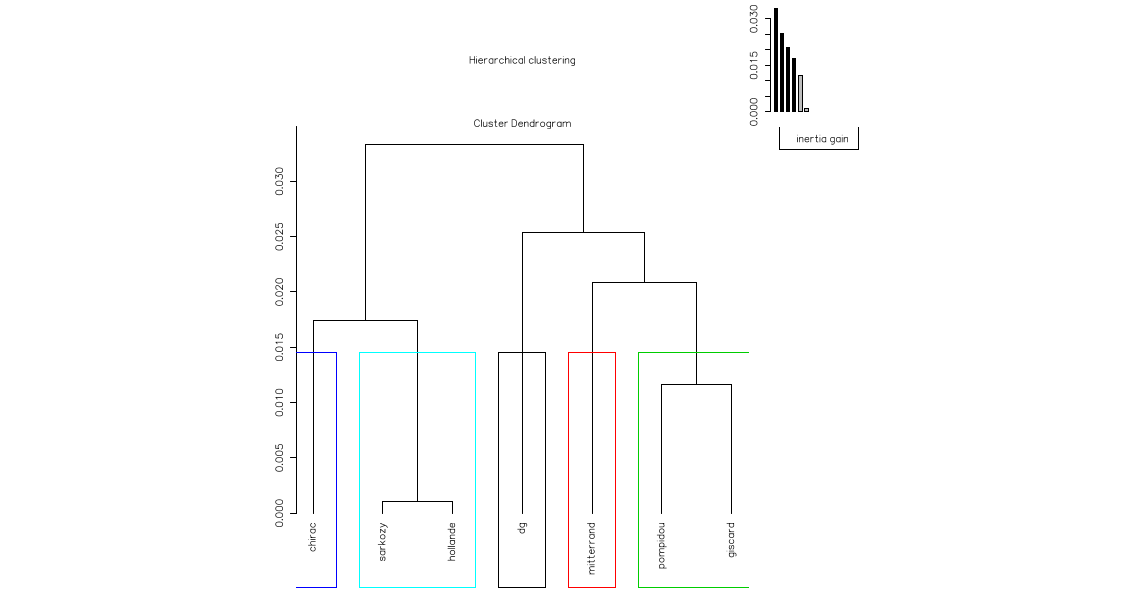
\includegraphics[width=1\linewidth]{img/cah.png}
		\caption{La \textsc{CAH} représentée par le vecteur fréquence des formes graphiques en utilisant la méthode d’agrégation \textit{ward} et une distance euclidienne.}
		\label{fig:ling_out_TAL}
	\end{figure}
\end{frame}
\begin{frame}[allowframebreaks]
		\printbibliography
\end{frame}

\begin{frame}{Licence}
	\centering
	{\small Le contenu de cette présentation est sous licence \texttt{CC-BY-NC-SA 4.0}\\Utilisation non commerciale -- Partage dans les mêmes conditions.\\}
	\href{https://creativecommons.org/licenses/by-nc-sa/4.0/deed.fr}{\ccbyncsa}
\end{frame}

\end{document}